% Q15：四个选项的圆弧图像；每个坐标系均按原图拓扑重绘，非比例图。
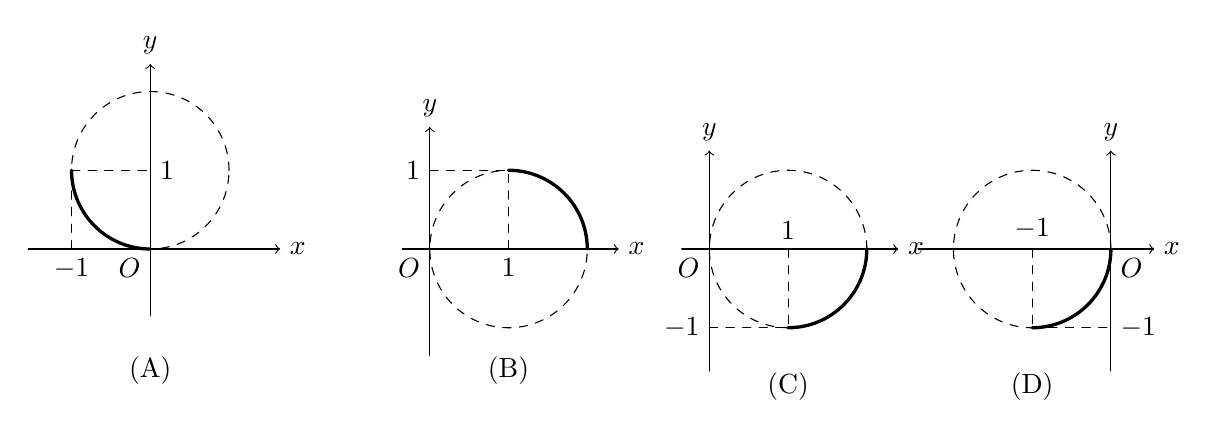
\begin{tikzpicture}[line cap=round,line join=round]
  % (A)
  \begin{scope}
    \draw[->] (-1.55,0)--(1.65,0) node[right] {$x$};
    \draw[->] (0,-0.85)--(0,2.35) node[above] {$y$};
    \draw[dashed] (0,1) circle[radius=1];
    \draw[dashed] (-1,0)--(-1,1) (-1,1)--(0,1);
    \draw[very thick] (0,1) ++(180:1) arc[start angle=180,end angle=270,radius=1];
    \node[below left] at (0,0) {$O$};
    \node[below] at (-1,0) {$-1$};
    \node[right] at (0,1) {$1$};
    \node at (0,-1.55) {(A)};
  \end{scope}

  % (B)
  \begin{scope}[xshift=3.55cm]
    \draw[->] (-0.35,0)--(2.4,0) node[right] {$x$};
    \draw[->] (0,-1.35)--(0,1.55) node[above] {$y$};
    \draw[dashed] (1,0) circle[radius=1];
    \draw[dashed] (0,1)--(1,1) (1,0)--(1,1);
    \draw[very thick] (1,0) ++(90:1) arc[start angle=90,end angle=0,radius=1];
    \node[below left] at (0,0) {$O$};
    \node[left] at (0,1) {$1$};
    \node[below] at (1,0) {$1$};
    \node at (1,-1.55) {(B)};
  \end{scope}

  % (C)
  \begin{scope}[xshift=7.1cm]
    \draw[->] (-0.35,0)--(2.4,0) node[right] {$x$};
    \draw[->] (0,-1.55)--(0,1.25) node[above] {$y$};
    \draw[dashed] (1,0) circle[radius=1];
    \draw[dashed] (0,-1)--(1,-1) (1,0)--(1,-1);
    \draw[very thick] (1,0) ++(270:1) arc[start angle=270,end angle=360,radius=1];
    \node[below left] at (0,0) {$O$};
    \node[above] at (1,0) {$1$};
    \node[left] at (0,-1) {$-1$};
    \node at (1,-1.75) {(C)};
  \end{scope}

  % (D)
  \begin{scope}[xshift=12.2cm]
    \draw[->] (-2.45,0)--(0.55,0) node[right] {$x$};
    \draw[->] (0,-1.55)--(0,1.25) node[above] {$y$};
    \draw[dashed] (-1,0) circle[radius=1];
    \draw[dashed] (-1,0)--(-1,-1) (-1,-1)--(0,-1);
    \draw[very thick] (-1,0) ++(270:1) arc[start angle=270,end angle=360,radius=1];
    \node[below right] at (0,0) {$O$};
    \node[above] at (-1,0) {$-1$};
    \node[right] at (0,-1) {$-1$};
    \node at (-1,-1.75) {(D)};
  \end{scope}
\end{tikzpicture}
